\begin{figure}[t]
\centering
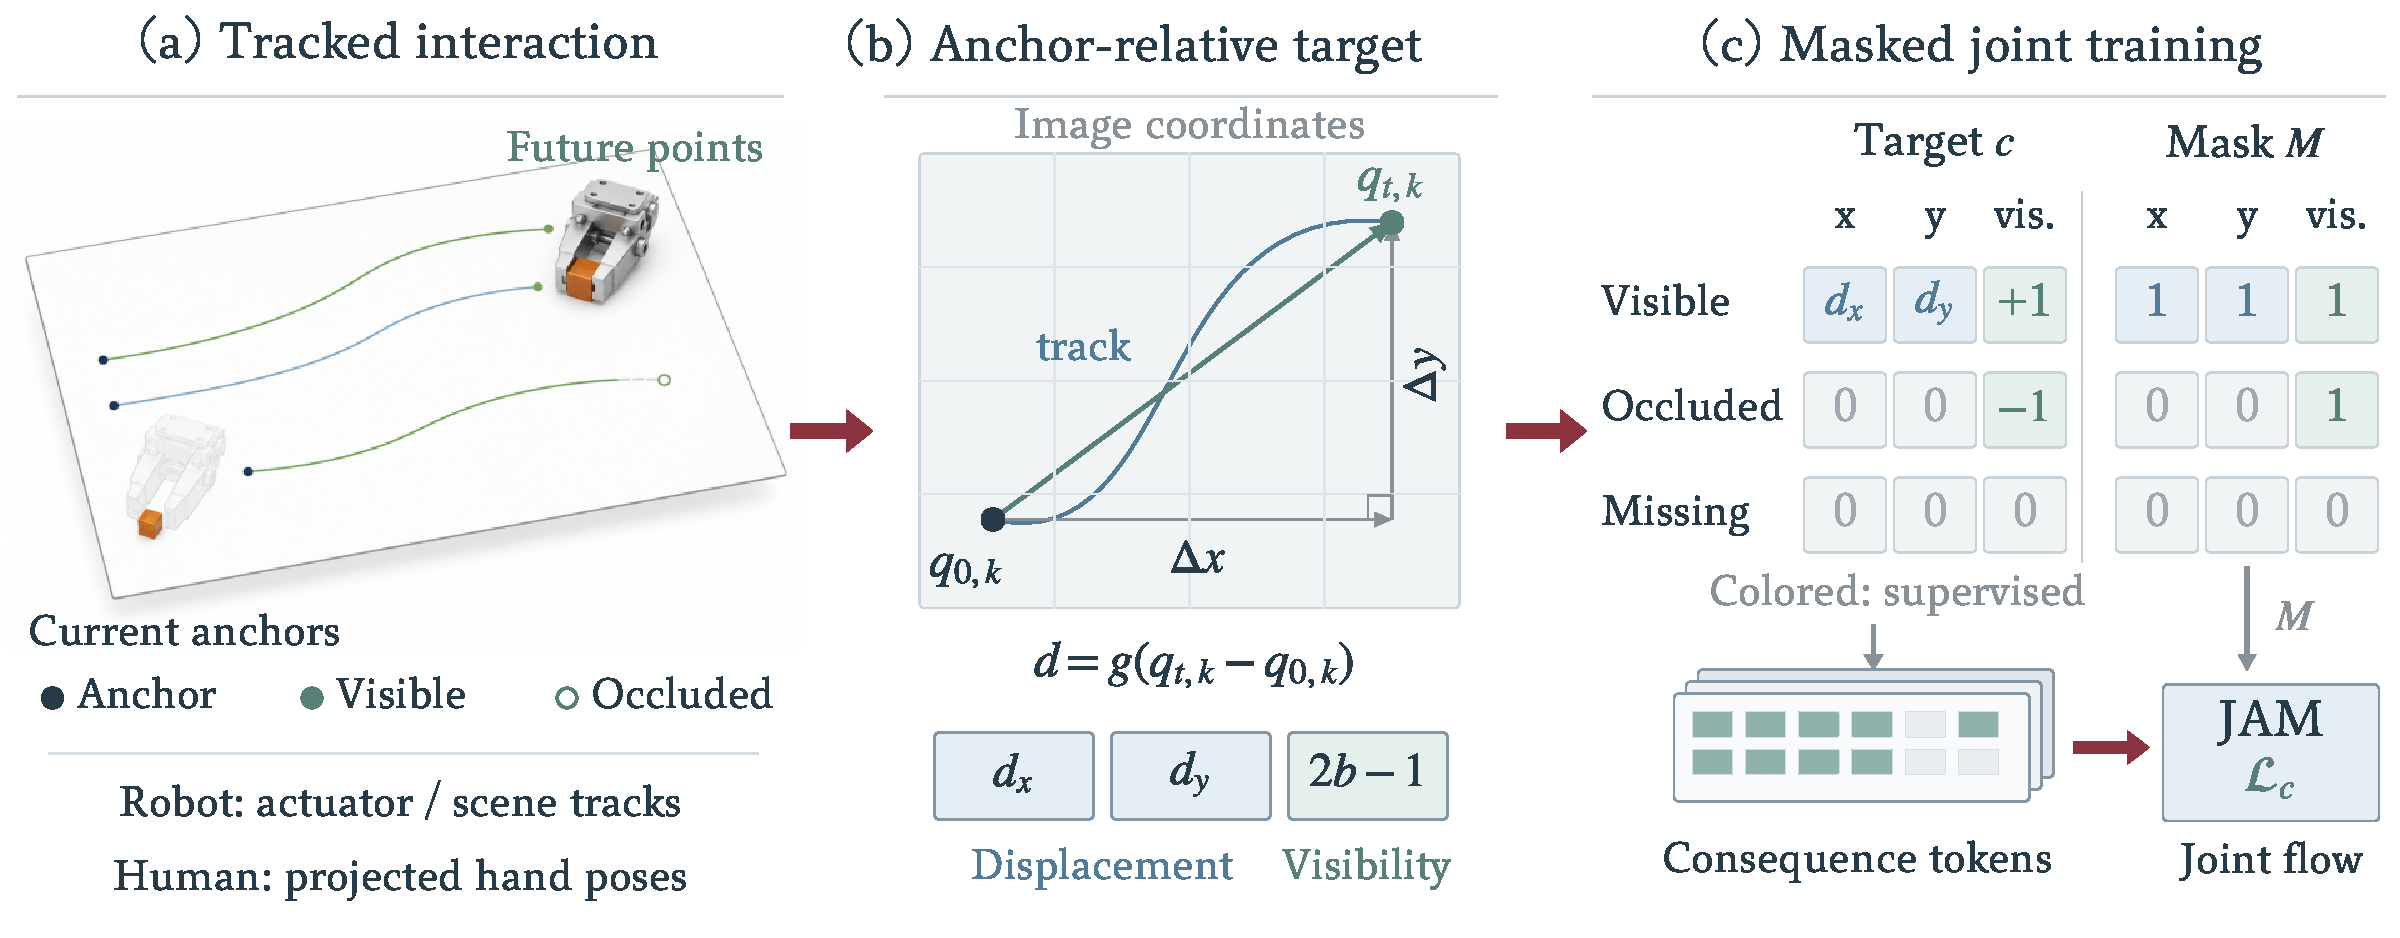
\includegraphics[width=\linewidth]{Figures/consequence_interface.pdf}
\caption{\textbf{What consequence supervision represents.}
(a) Tracks connect current anchors to future image positions. Robot labels can combine actuator
and scene tracks; the active human adapter projects supplied hand poses.
(b) The target contains gain-scaled displacement $d$ and observability.
(c) Binary visibility examples distinguish visible points, occluded points, and missing slots.
An occluded point retains visibility supervision; its stored zero displacement is masked.
A missing slot is fully masked. Consequence tokens enter JAM's joint flow objective, with mask $M$
selecting supervised coordinates. The interaction and mask cases are explanatory schematics.}
\label{fig:consequence}
\end{figure}
